
%
%  $Description: Author guidelines and sample document in LaTeX 2.09$
%
%  $Author: ienne $
%  $Date: 1995/09/15 15:20:59 $
%  $Revision: 1.4 $
%

%\documentclass[times, 10pt,twocolumn]{article}
\documentclass[conference]{IEEEtran}
\input{macros}
%\usepackage{latex8}
%\usepackage{times}

%\documentstyle[times,art10,twocolumn,latex8]{article}

%-------------------------------------------------------------------------
% take the % away on next line to produce the final camera-ready version
\pagestyle{empty}

%-------------------------------------------------------------------------
\begin{document}

\title{SpotWeb: Detecting Framework Hotspots and Coldspots via Mining Open Source Code on the Web}

\author{Suresh Thummalapenta\\
Department of Computer Science\\ North Carolina State University \\
Raleigh, USA\\ sthumma@ncsu.edu\\
% For a paper whose authors are all at the same institution,
% omit the following lines up until the closing ``}''.
% Additional authors and addresses can be added with ``\and'',
% just like the second author.
\and
Tao Xie\\
Department of Computer Science\\ North Carolina State University \\
Raleigh, USA\\ xie@csc.ncsu.edu\\
}

\maketitle
\thispagestyle{empty}

\begin{abstract}
Code Search Engines (CSE) can serve as powerful resources of open
source code, as they can search in billions of lines of open source
code available on the web. The strength of CSEs can be used for
several tasks like searching relevant code samples, identifying
hotspots, and finding bugs. However, the major limitations in using
CSEs for these tasks are that the returned samples are too many and
they are often partial. Our framework addresses the preceding
limitations and thereby helps in using CSEs for these tasks. We
showed the effectiveness of our framework with two tools developed
based on our framework.

\Comment{CSEs are often used by programmers to search for relevant
code samples from publicly accessible source code. However, CSEs are not quite
helpful in practice because the number of returned samples are too many and
the desired code sample is often not available among the first several results.
Apart from using CSEs for searching relevant code samples, CSEs can also be used
for several other applications like identifying framework hotspots and finding bugs
in software. Exploiting CSEs for these applications requires analysis of
the code samples returned by CSEs. This analysis is non-trivial because the code samples
returned by CSEs are often partial.\Comment{, as CSEs retrieve
only source files with usages of the given query instead of entire projects.}
In this paper, we propose an extensible framework that addresses the preceding limitations
and thereby helps in exploiting CSEs for several applications that can help improve the
productivity of programmers. Our framework performs static analysis over code samples gathered from a CSE by
using several heuristics and transforms those samples into graph representations that can be directly
used for other applications. }
\end{abstract}

\Comment{
\vspace{1mm} \noindent {\bf Categories and Subject Descriptors:}
D.2.3 {[Software Engineering]}: {Coding Tools and
Techniques---\emph{Object-oriented programming}}; D.2.6 {[Software Engineering]}: {Programming
Environments---\emph{Integrated environments}};

\vspace{1mm} \noindent {\bf General Terms:} Languages,
Experimentation.

\vspace{1mm} \noindent {\bf Keywords:} Hotspots, Coldspots, Code search
engine, Code reuse
}
%-------------------------------------------------------------------------
\section{Introduction}
\label{sec:introduction}

The primary goal of software development is to deliver high-quality
software efficiently and in the least amount of time whenever
possible. To achieve the preceding goal, programmers often want to
reuse existing frameworks or libraries instead of developing similar
code artifacts from scratch. The challenging aspect for
programmers in reusing the existing frameworks or libraries is to
understand the usage of Application Programming Interfaces (APIs)
exposed by those frameworks or libraries, because many of the
existing frameworks or libraries are not well-documented. Even when
such documentations exist, they are often outdated~\cite{document:leth}.

In general, the reuse of existing frameworks or libraries involve
instantiation of several object types of those frameworks or
libraries. For example, consider the programming task of parsing
code in a dirty editor (editor whose content is not yet saved) of
the Eclipse IDE framework. As a dirty editor is represented as an
object of the \CodeIn{IEditorPart} type and the programmer needs an
object of \CodeIn{ICompilationUnit} for parsing, the programmer has
to identify a method sequence that takes the \CodeIn{IEditorPart} object
as input and results in an object of \CodeIn{ICompilationUnit}. One
such possible method sequence is shown below:

\begin{CodeOut}
\begin{alltt}
IEditorPart iep = ...
IEditorInput editorInp = iep.getEditorInput();
IWorkingCopyManager wcm = JavaUI.getWorkingCopyManager();
ICompilationUnit icu = wcm.getWorkingCopy(editorInp);
\end{alltt}
\end{CodeOut}

The code sample shown above exhibits the difficulties faced by
programmers in reusing the existing frameworks or libraries. A
programmer unfamiliar to Eclipse may take
long time to identify that an \CodeIn{IWorkingCopyManager} object 
is needed for getting the
\CodeIn{ICompilationUnit} object from an object of the
\CodeIn{IEditorInput} type. Furthermore, it is not trivial to find
an appropriate way of instantiating the
\CodeIn{IWorkingCopyManager} object as the instantiation requires a static
method invocation on the \CodeIn{JavaUI} class.

In many such situations, programmers know what type of object that
they need to instantiate (like \CodeIn{ICompilationUnit}), but do
not know how to write code to get that object from a known object
type (like \CodeIn{IEditorPart}). For simplicity, we refer the known
object type as \emph{Source} and the required object type as
\emph{Destination}. Therefore, the proposed problem can be
translated to a query of the form ``\emph{Source} $\rightarrow$
\emph{Destination}''. There are several existing
approaches~\cite{prospector:jungloid, strathcona:se, xsnippet:saha}
that address the described problem. But the common issue faced by
these existing approaches is that the scope of these approaches is
limited to the information available in a fixed (often small) set of
applications reusing the frameworks or libraries of interest.
%-------------------------------------------------------------------------
\begin{figure*}[t]
\begin{CodeOut}
\begin{alltt}
\hspace*{0.6in}01:\textbf{FileName}:0\_UserBean.java \textbf{MethodName}:ingest  \textbf{Rank}:1 \textbf{NumberOfOccurrences}:6
\hspace*{0.6in}02:QueueConnectionFactory,createQueueConnection() \textbf{ReturnType}:QueueConnection
\hspace*{0.6in}03:QueueConnection,createQueueSession(boolean,Session.AUTO\_ACKNOWLEDGE) \textbf{ReturnType}:QueueSession
\hspace*{0.6in}04:QueueSession,createSender(Queue) \textbf{ReturnType}:QueueSender
\end{alltt}
\end{CodeOut}
\vspace*{-4ex} \Caption{\label{fig:sampleoutput} Method sequence
suggested by PARSEWeb.}
%-------------------------------------------------------------------------
%\begin{figure}[t]
\begin{CodeOut}
\begin{alltt}
\hspace*{0.6in}01:QueueConnectionFactory qcf;
\hspace*{0.6in}02:QueueConnection queueConn = qcf.createQueueConnection();
\hspace*{0.6in}03:QueueSession qs = queueConn.createQueueSession(true,Session.AUTO\_ACKNOWLEDGE);
\hspace*{0.6in}04:QueueSender queueSender = qs.createSender(new Queue());
\end{alltt}
\end{CodeOut}\vspace*{-4ex}
\Caption{\label{fig:javacode} Equivalent Java code for the method sequence suggested by PARSEWeb.} \vspace*{-3ex}
\end{figure*}
%-------------------------------------------------------------------------
Many code search engines (CSE) such as Google~\cite{GCSE} and
Koders~\cite{KODERS}\Comment{, and Krugle~\cite{KRUGLE}} are
available on the web. These CSEs can be used to assist programmers
by providing relevant code examples with usages of the given query
from a large number of publicly accessible source code repositories.
For the preceding example, programmers can issue the query
``\CodeIn{IEditorPart} \CodeIn{ICompilationUnit}'' to gather
relevant code samples with usages of the object types
\CodeIn{IEditorPart} and \CodeIn{ICompilationUnit}. However, these
CSEs are not quite helpful in addressing the described problem
because we observed that Google Code Search Engine (GCSE)
~\cite{GCSE} returns nearly $100$ results for this
query and the desired method sequence shown above is present in the
$25^{th}$ source file among those results.

Our approach addresses the described problem by accepting
queries of the form ``\emph{Source} $\rightarrow$
\emph{Destination}'' and suggests frequently used Method-Invocation
Sequences (MIS) that can transform an object of the \emph{Source}
type to an object of the \emph{Destination} type. Our approach also
suggests relevant code samples that are extracted from a large
number of publicly accessible source code repositories. These
suggested MISs along with the code samples can help programmers in
addressing the described problem and thereby help reduce
programmers' effort in reusing existing frameworks or libraries.

We have implemented the proposed approach with a tool called
PARSEWeb for helping reuse Java code. PARSEWeb interacts with
GCSE~\cite{GCSE} to search for code samples with the usages of the
given \emph{Source} and \emph{Destination} object types, and
downloads the code example results to form a local source code
repository. PARSEWeb analyzes the local source code repository to
extract different MISs and clusters similar MISs using a
sequence postprocessor. These extracted MISs can serve as a solution for
the given query. PARSEWeb also sorts the final set of MISs using
several ranking heuristics. PARSEWeb uses an additional heuristic
called query splitting that helps address the problem where
code samples for the given query are split among different source
files.

This paper makes the following main contributions:\vspace*{-1ex}
\begin{itemize}
\item An approach for reducing programmers' effort while reusing existing frameworks or libraries by providing frequently used MISs and relevant code samples.
\item A technique for collecting relevant code samples dynamically from the web. This contribution has an added advantage of not limiting the scope of the approach to any specific set of frameworks or libraries.
\item A technique for analyzing partial code samples through Abstract Syntax Trees (AST) and Directed Acyclic Graphs (DAG) that can handle control-flow information and method inlining.
\item An Eclipse plugin tool implemented for the proposed approach
and several evaluations to assess the effectiveness of the tool.
\end{itemize}

The rest of the paper is organized as follows. Section
~\ref{sec:example} explains the approach through an example.
Section~\ref{sec:relatedwork} presents related work.
Section~\ref{sec:summary} describes key aspects of the approach.
Section~\ref{sec:implementation} describes implementation details.
Section~\ref{sec:evaluation} discusses evaluation results.
Section~\ref{sec:discussion} discusses limitations and future work.
Finally, Section~\ref{sec:conclusion} concludes.\vspace*{-1ex}
%-------------------------------------------------------------------------

\section{Example}
\label{sec:example}

\begin{figure*}[t]
\centering
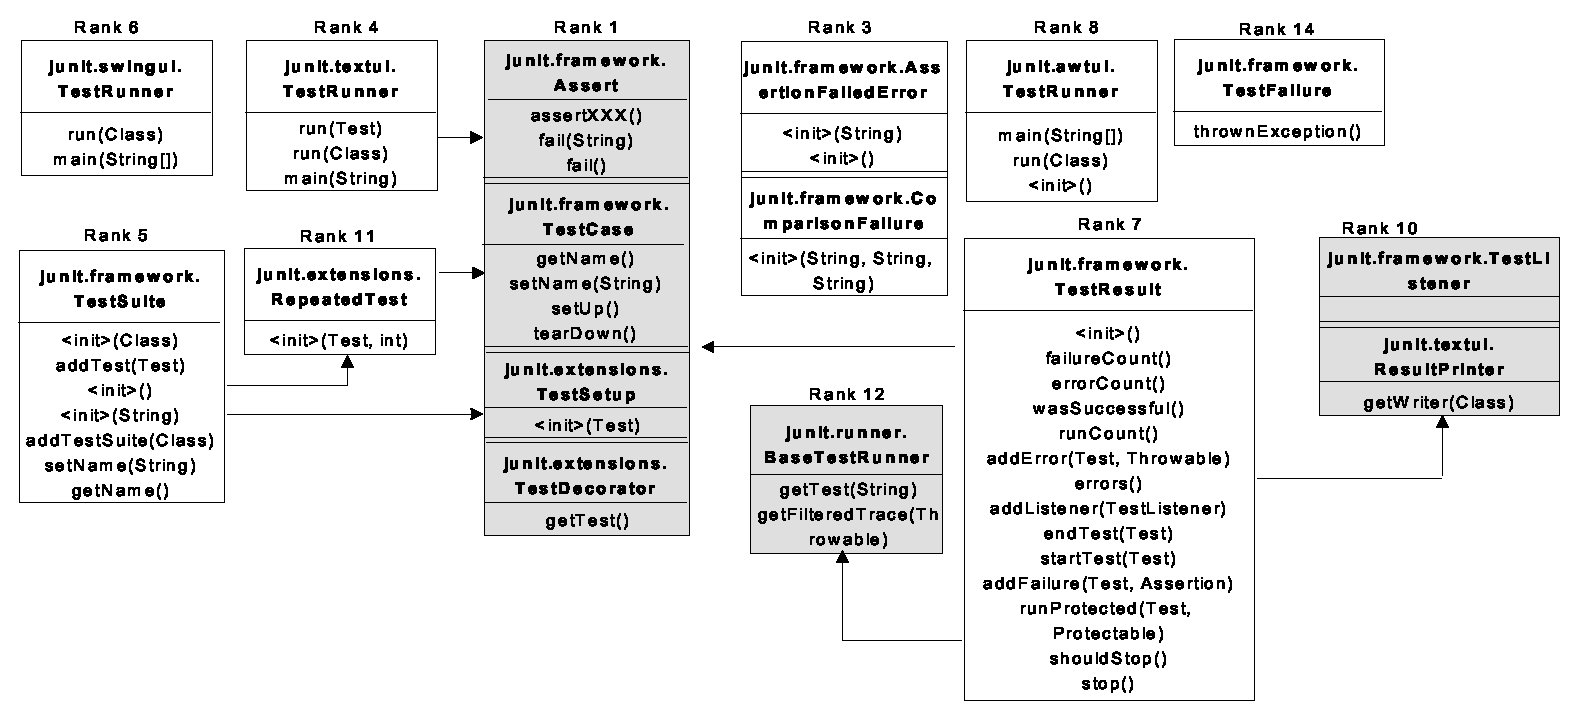
\includegraphics[scale=0.68,clip]{figs/examplehotspot_final.eps}
\caption{Hotspot hierarchies identified for the JUnit framework} \label{fig:hotspotexample}
\end{figure*}

We next use an example to explain our approach and show how the detected
hotspots and coldspots can be used by the framework users. We use JUnit~\cite{JUNIT}, the
\emph{de facto} standard unit testing framework for Java, 
as an illustrative example for explaining our approach.

SpotWeb accepts an input framework, say JUnit, and extracts
\emph{FrameworkInfo} from the framework. The
\emph{FrameworkInfo} includes all classes, all interfaces, public
or protected methods of each class and interface, and inheritance
hierarchy among classes or interfaces of the framework. SpotWeb also captures
the constants defined by the input framework. SpotWeb
constructs different queries for each class or interface and
interacts with a CSE such as Google code search~\cite{GCSE} to
gather relevant code examples from existing open source projects that
reuse the classes of the input framework. For example, SpotWeb constructs
a query such as ``\CodeIn{lang:java junit.framework.TestSuite}'' for
gathering relevant code examples of the \CodeIn{TestSuite} class. These
gathered code examples are referred as a \emph{LocalRepository} for
the input framework. SpotWeb analyzes gathered code examples
statically and computes \emph{UsageMetrics} for classes, interfaces,
and public or protected methods of all classes and interfaces. For
example, the \emph{UsageMetrics} computed for the \CodeIn{TestSuite}
class show that the class is instantiated for 165 times and is
extended for 32 times. Similarly, the \emph{UsageMetrics} computed
for the method \CodeIn{addTest} of the \CodeIn{TestSuite} class show
that the method is invoked for 95 times. SpotWeb also gathers code
examples for each class or method and stores these code examples in
a repository, referred as \emph{ExampleDB}. Then SpotWeb uses the
algorithm shown in Figure~\ref{alg:hotspotalgo} for detecting
hotspots from the computed \emph{UsageMetrics}.

Initially, SpotWeb ranks methods in a non-ascending order based on
their \emph{UsageMetrics} and uses a threshold percentage $HT$ to
detect hotspot methods: the methods in the top $HT$ percentage with
a non-zero \emph{UsageMetrics} are detected as hotspot methods. 
The detected hotspot methods are then
grouped into their declaring classes, detected as hotspot classes.
These hotspot classes are ranked based on the minimum rank of the
hotspot methods declared by these classes. SpotWeb classifies the
hotspot classes into two categories (templates and hooks) based on
heuristics described in Step 4 of the algorithm shown in Figure~\ref{alg:hotspotalgo}. The hotspot classes of each
category are further grouped into hierarchies based on their
inheritance relationships. For example, SpotWeb detected classes
\CodeIn{Assert} and \CodeIn{TestCase} as hook hotspots in the JUnit
framework. As \CodeIn{TestCase} class extends \CodeIn{Assert} class,
SpotWeb groups both the classes into the same hierarchy. SpotWeb
assigns a rank to each hierarchy based on the minimum rank of the
hotspot classes contained in the hierarchy. For example, consider
that the \CodeIn{Assert} class has Rank 1 and the \CodeIn{TestCase}
class has Rank 2, then the grouped hierarchy of the
\CodeIn{Assert} and \CodeIn{TestCase} classes is assigned with Rank
1. The rank attribute uniquely identifies a hierarchy among all
other hierarchies. Hierarchies with smaller ranks have higher preference
or importance to the hierarchies with larger ranks.

Figure~\ref{fig:hotspotexample} shows the hotspot hierarchies detected for the JUnit
framework. The figure also shows ranks assigned to each hierarchy.
As the rank attribute uniquely identifies a hierarchy, we use the
rank as an identity for describing a hierarchy.
Each hierarchy includes one or more hotspot classes and is shown as pairs of class and its methods.
For example, Hierarchy 1 (hierarchy with Rank 1) has classes \CodeIn{Assert}, \CodeIn{TestCase}, \CodeIn{TestSetup},
and \CodeIn{TestDecorator}. We show template hierarchies in white and hook hierarchies in gray.
For example, Hierarchy 1 is a hook hierarchy and Hierarchy 3 is a template hierarchy.

Methods inside each class of a hierarchy are sorted
based on their computed \emph{UsageMetrics}. Sorting methods of a class
can assist the framework users in quickly identifying the methods that are often
used inside a given hotspot class. For example, consider the \CodeIn{TestSuite} class
shown in Hierarchy 5. The \CodeIn{TestSuite} class has three constructors \CodeIn{<init>(Class)},
\CodeIn{<init>()}, and \CodeIn{<init>(String)}. However, the \CodeIn{<init>(Class)} constructor
is often used compared to the other two constructors. Due to space limit,
we show all assertion methods such as \CodeIn{assertEquals} and \CodeIn{assertTrue}
of the class \CodeIn{Assert} of Hierarchy 1 as \CodeIn{assertXXX}.

The figure also displays dependencies among hotspot hierarchies
(shown as arrows between hierarchies). SpotWeb captures the
usage relationships among hotspot classes through dependencies.
For example, Hierarchy $5$ has a
\CodeIn{TEMPLATE\_HOOK} dependency with Hierarchy $1$. This
dependency indicates that to reuse methods such as \CodeIn{addTest}
of the class \CodeIn{TestSuite} in Hierarchy 5, the user has to
define a new behavior for the classes in Hierarchy $1$.

\begin{figure}[t]
\begin{CodeOut}
\begin{alltt}
01:public class SRDAOTestCase 
02:\hspace*{0.4in}extends TestCase \{
03:\hspace*{0.1in}private SRDAO dao = null;...
04:\hspace*{0.1in}public SRDAOTestCase() \{
05:\hspace*{0.3in}super(); ... 
06:\hspace*{0.1in}\}
07:\hspace*{0.1in}protected void setUp() throws Exception \{
08:\hspace*{0.3in}...
09:\hspace*{0.3in}dao = (SRDAO)context.getBean("SRDAO");
10:\hspace*{0.3in}...
11:\hspace*{0.1in}\}
12:\hspace*{0.1in}public void tearDown() throws Exception \{
13:\hspace*{0.3in}dao = null; 
14:\hspace*{0.1in}\}
15:\hspace*{0.1in}public void testF() \{ ... \}
16:\hspace*{0.1in}public void testB() \{ ... \}
17:\hspace*{0.1in}...
18:\}
\end{alltt}
\end{CodeOut}
\Caption{\label{fig:hcodeexample} Suggested code example for the hook class \CodeIn{TestCase}.}
\begin{CodeOut}
\begin{alltt}
01:public class MyTestSuite \{ 
02:\hspace*{0.1in}...
03:\hspace*{0.1in}public static Test suite() \{
04:\hspace*{0.3in}TestSuite suite = new TestSuite("axis");
05:\hspace*{0.3in}suite.addTest(new SRDAOTestCase());
06:\hspace*{0.3in}return suite;
07:\hspace*{0.1in}\}
08:\hspace*{0.1in}...
09:\}
\end{alltt}
\end{CodeOut}
\Caption{\label{fig:tcodeexample} Suggested code example for the template class \CodeIn{TestSuite}.}
\end{figure}

We next describe how the hotspots detected by SpotWeb can be used by
the framework users to reuse classes of the JUnit framework. After reviewing
the hotspots shown in Figure~\ref{fig:hotspotexample}, consider that
a framework user wants to start with the method \CodeIn{addTest} of
the template class \CodeIn{TestSuite} in Hierarchy 5.
Figure~\ref{fig:hotspotexample} shows that Hierarchy 5 of the
\CodeIn{TestSuite} class has a \CodeIn{TEMPLATE\_HOOK} dependency
with the Hierarchy 1. This dependency indicates that the user may
need to define a new behavior for the associated hook hierarchy.
SpotWeb recommends the code example shown in
Figure~\ref{fig:hcodeexample} for the hook class \CodeIn{TestCase},
which is part of Hierarchy 1. The code example exhibits several
aspects that need to be handled by the user while extending the
\CodeIn{TestCase} class. For example, in the \CodeIn{setUp} method,
the user can write code for setting up the environment such as
instantiating necessary variables, and in the \CodeIn{tearDown}
method, the user can destroy the created variables. In addition, the code
example shows that names of the test methods in the extended class
of the \CodeIn{TestCase} class should start with the prefix \CodeIn{test}.
SpotWeb also recommends a code example for the \CodeIn{addTest} method and
the recommended code example is shown in
Figure~\ref{fig:tcodeexample}. The code example shows that the user
has to create an instance of the \CodeIn{TestSuite} class and then
add test cases through the \CodeIn{addTest} method.

An API class or method is identified as a coldspot if that class or method is neither
used directly nor used indirectly by gathered code examples. The complete
algorithm used for detecting coldspots is shown in Figure~\ref{alg:coldspotalg}. SpotWeb identified $20$
classes such as \CodeIn{Swapper}, \CodeIn{TestRunListener}, and \CodeIn{ExceptionTestCase} as coldspots
in the JUnit framework. However, coldspots are only suggestions
for users unfamiliar to that framework and SpotWeb does not intend to recommend users not to reuse
those coldspot classes. Sometimes, coldspots can also be helpful to
the framework developers in distributing their maintenance efforts, because the framework
developers can give a low preference to the coldspot classes.

\section{Approach}
\label{sec:approach}
\begin{figure}[t]
\centering
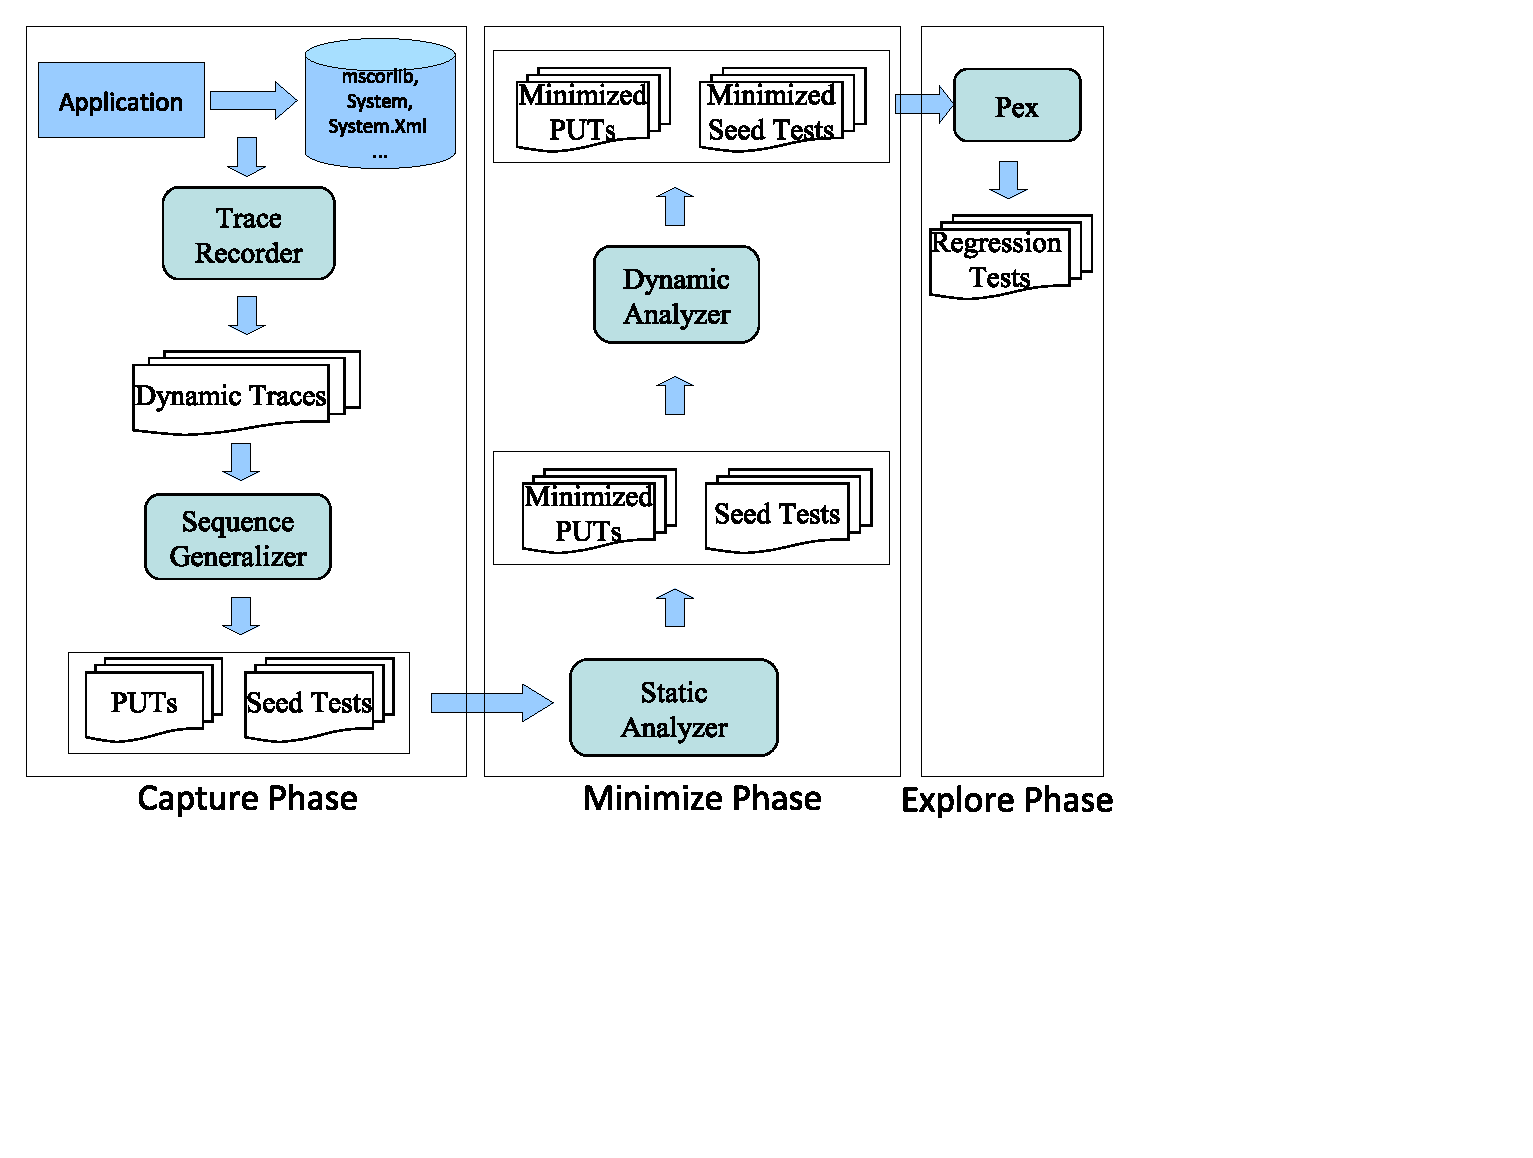
\includegraphics[scale=1,clip]{figure/approach.eps}\vspace*{-3ex}
 \caption{Overview of TeMaAPI}\vspace*{-4ex}
 \label{fig:approach}
\end{figure}
Given a migration tool between Java and C\#, TeMaAPI generates various test cases to reveal different behaviors of the tool's API mapping relations.
Figure~\ref{fig:approach} shows the overview of TeMaAPI.


%-------------------------------------------------------------------
\subsection{Generating client code}
\label{sec:approach:generating}
Given a migration tool, TeMaAPI first extracts its validate mapping relations of APIs. It is challenging to extract such mapping relations directly from a migration tool for two factors: (1) different migration tools may follow different styles to describe API mapping relations. For example, as shown in Section~\ref{sec:introduction}, the API mapping relations of Java2CSharp are described in its mapping files, but the API mapping relations of sharpen are hard-coded in its source files. (2) commercial migration tools typically hide their API mapping relations in binary files. Due to the two factors, TeMaAPI does not extract API mapping relations directly from a migration tool, but chooses to analyze translated code of a migration tool. We choose to use migration tools to translate simple client code instead of existing projects for two considerations: (1) Existing projects typically use quite a small set of APIs, so many API mapping relations may be not covered; (2) a single method of an existing project may use multiple APIs, so it may be difficult to analyze which APIs are not mapped. For the preceding consideration, TeMaAPI chooses to generate client code instead of using existing client code.

TeMaAPI relies on the reflection technique~\cite{maes1987concepts} provided by both Java and C\# to generate client code for translation.

\textbf{Static fields.} Given a public static field \CodeIn{f} of a class \CodeIn{C} whose type is \CodeIn{T}, TeMaAPI generates a getter as follows:
\begin{CodeOut}%\vspace*{-2ex}
\begin{alltt}
 public T TestGet|f.name||no|()\{ return C.f; \}
\end{alltt}
\end{CodeOut}

If \CodeIn{f} is not a constant, TeMaAPI generates a setter as follows:
\begin{CodeOut}%\vspace*{-2ex}
\begin{alltt}
 public void TestSet|f.name||no|(T v)\{ C.f = v; \}
\end{alltt}
\end{CodeOut}

\textbf{Non-static fields.} Given a public non-static field \CodeIn{f} of a class \CodeIn{C} whose type is \CodeIn{T}, TeMaAPI generates a getter for each constructor \CodeIn{C(T1\ p1,\ldots, Tn\ pn)} of \CodeIn{C} as follows:
\begin{CodeOut}%\vspace*{-2ex}
\begin{alltt}
 public T TestGet|f.name||no|(T1\ c1,\ldots, Tn\ cn)\{
    C obj = new C(c1,\ldots, cn);
    return obj.f; \}
\end{alltt}
\end{CodeOut}

If \CodeIn{f} is not a constant, TeMaAPI generates a setter as follows:
\begin{CodeOut}%\vspace*{-2ex}
\begin{alltt}
 public void TestSet|f.name||no|(T1\ c1,\ldots, Tn\ cn)\{
   C obj = new C(c1,\ldots, cn);
   obj.f = v; \}
\end{alltt}
\end{CodeOut}

In the preceding code, ``\CodeIn{|f.name|}'' denotes the name of \CodeIn{f}, and ``\CodeIn{|no|}'' denotes the corresponding number of generated client-code method.

\textbf{Static methods.} Given a public static method \CodeIn{m(T1\ p1,\ldots,Tn\ pn)} of a class \CodeIn{C} whose return type is \CodeIn{Tm}, TeMaAPI generates a client-code method as follows:
\begin{CodeOut}%\vspace*{-2ex}
\begin{alltt}
 public Tm Test|m.name||no|(T1\ m1,\ldots, Tn\ mn)\{
   return C.m(m1,\ldots, mn); \}
\end{alltt}
\end{CodeOut}

\textbf{Non-static methods.} Given a public non-static method \CodeIn{m(T1\ p1,\ldots,Tn\ pn)} of a class \CodeIn{C} whose return type is \CodeIn{Tm}, TeMaAPI generates a client-code method for each constructor \CodeIn{C(Tv\ pv,\ldots, Tt\ pt)} of \CodeIn{C} as follows:
\begin{CodeOut}%\vspace*{-2ex}
\begin{alltt}
 public Tm Test|m.name||no|(T1\ m1,\ldots, Tn\ mn,
                            Tv cv, \ldots, Tt ct)\{
   C obj = new C(cv,\ldots, ct);
   return obj.m(m1,\ldots, mn); \}
\end{alltt}
\end{CodeOut}

In the preceding code, ``\CodeIn{|m.name|}'' denotes the name of \CodeIn{m(T1\ p1,\ldots,Tn\ pn)}.

TeMaAPI ignores generic methods for simplicity, and organizes all generated client code methods by the corresponding class $C$. For a migration tool that translates from Java to C\#, TeMaAPI generates client code in Java as shown by the solid line of Figure~\ref{fig:approach}, and for a migration tool that translates from C\# to Java, TeMaAPI generates client code in C\# as shown by the dotted line of Figure~\ref{fig:approach}. When TeMaAPI generates client code in C\#, it ignores \CodeIn{unsafe} and \CodeIn{delegate} methods and methods whose parameters are marked as \CodeIn{our} or \CodeIn{ref}. Java does not have corresponding keywords, so there are typically no mapped methods in Java for these C\# methods. After TeMaAPI generate client-code methods, we translate them using a migration tool under experiments.


%-----------------------------------------------------------------
\subsection{Analyzing Generated Methods}
\label{sec:approach:analyzing}
Translated code typically contain many compilation errors since a migration tool typically cannot cover mapping relations of all APIs. TeMaAPI then analyzes translated code for validate API mapping relations of the migration tool. To achieve this, TeMaAPI first remove all translated methods with compilation errors. For translated methods in Java, TeMaAPI implements a Eclipse plug-in that uses on Eclipse JDT compiler\footnote{\url{http://www.eclipse.org/jdt/}} for the list of compilation errors. For translated methods in C\#, TeMaAPI implements a Visual Studio.Net add-in to retrieve the list of compilation errors from the error-list view of Visual Studio.Net. Both Eclipse JDT compiler and Visual Studio.Net cannot list all methods with compilation errors in a single build. After each iteration of removing methods, TeMaAPI re-build these methods until it removes all methods with compilation errors.

After methods with compilation errors are removed, TeMaAPI compares generated code with translated code for the validate API mapping relations of a migration tool. Based on translated code and validate API mapping, TeMaAPI removes generated methods whose corresponding translated methods have compilation errors. We refer to those removing client-code methods as safe methods.

%-----------------------------------------------------------
\subsection{Finding Different Behaviors}
\label{sec:approach:behavior}
In the final step, TeMaAPI generates test cases to detect different behaviors of API mapping relations. An alternative approach is to use existing test cases in two languages. For example, lucene\footnote{\url{http://lucene.apache.org}} has both a Java version and a C\# version. It is feasible to use these test cases to reveal some different behaviors, but such test cases typically cover only a small set of APIs. Some test suites such as Java Compatibility Kit (JCK)\footnote{\url{http://jck.dev.java.net}} cover most APIs of a language. However, translating such a test suite from one language into another language may introduce many compilation errors and defects. A test method may use many APIs, so even if the API under test can be translated correctly, the test method cannot be translated correctly since other APIs are not mapped. As a result, we choose to translating existing test suites as a supplement of our approach.

\subsubsection{Generating Test Cases}
\label{sec:approach:behavior:generating}
For each safe method in Java, we use Randoop~\cite{pacheco2007feedback} to generate its test cases. For each safe method in C\#, we use Pex~\cite{tillmann2008pex} to generate its test cases. TeMaAPI then executes generated test cases, and records the inputs, the output, and the thrown exception of each test case as a file.

Based on the file, TeMaAPI generates Junit\footnote{\url{http://www.junit.org/}} or Nunit\footnote{\url{http://www.nunit.org/}} test cases to ensure each mapped API produce the same output give the same inputs. For example, Pex generates a test case whose input is \CodeIn{m0 = false} for the \CodeIn{TestvalueOf57} method in C\# as shown in Section~\ref{sec:example}, and after executing the output of the test case is ``False''. Based on the input and the output of this test case, TeMaAPI generates a Junit test case as follows:

\begin{CodeOut}%\vspace*{-2ex}
\begin{alltt}
 @Test
 public void testvalueOf64zhh0()\{
   sketch.Test_java_lang_String obj =
                       new sketch.Test_java_lang_String();
   boolean m0 = false;
   Assert.assertEquals("False", obj.testvalueOf64(m0));\}
\end{alltt}
\end{CodeOut}

This Junit test case fails since the preceding \CodeIn{testvalueOf64zhh} method produces ``false'' instead of ``False''. From this failed Junit test case, TeMaAPI detects that the \CodeIn{java.lang.String.valueOf (Object)} method in Java has different behaviors with its mapped C\# methods if inputs are boolean values.

In some cases, executing a test case does not produce outputs but exceptions. For example, Pex also generates a test case whose input is \CodeIn{m0 = null} for the \CodeIn{TestvalueOf57} method in C\# as shown in Section~\ref{sec:example}, after executing it throws \CodeIn{NullReferenceException}. TeMaAPI finds that the \CodeIn{NullPointerException} class in C\# is mapped to the \CodeIn{NullPointerException} class in Java in the validate API mapping relations, and generates a Junit test case based on the preceding mapping relation and input as follows:

\begin{CodeOut}%\vspace*{-2ex}
\begin{alltt}
 @Test
 public void testvalueOf64zhh3()\{
   try\{
     sketch.Test_java_lang_String obj =
                       new sketch.Test_java_lang_String();
     boolean m0 = null;
     obj.testvalueOf64(m0);\}
   \}catch(java.lang.NullPointerException e)\{
       Assert.assertTrue(true);
       return;
   \}
   Assert.assertTrue(false);\}
\end{alltt}
\end{CodeOut}

This Junit test case also fails since given a null input, the preceding \CodeIn{testvalueOf64} method does not throw any exceptions. From this failed Junit test case, TeMaAPI detects that the \CodeIn{java.lang. String.valueOf(Object)} method in Java has different behaviors with its mapped C\# methods if inputs are null pointers.

\subsubsection{Translating Existing Test Cases}
\label{sec:approach:behavior:jck}

Each generated client-code method uses only one fields or methods provided by API libraries, and may lose some complicated behaviors even if test cases satisfy the round-trip criterion. To test those complicated behaviors, we introduce JCK that covers many complicated behaviors of Java APIs. JCK is a test suite provided by Sun to ensure compatibility of Java platforms, and it covers most standard APIs of J2SE. However, JCK implements many internal classes to collect the results of executed test cases. If a migration tool cannot correctly translate one of these classes, all translated test cases may have compilation errors or defects. In addition, JCK is released under read-only source license\footnote{\url{http://tinyurl.com/33x9fo6}}, so many such internal classes are not shipped and it has many compilation errors. To increase the chance of migrating JCK, TeMaAPI first replaces those internal classes with the classes of Junit. For example, one test method for \CodeIn{java.io.File.delete()} in JCK is as follows:

\begin{CodeOut}%\vspace*{-2ex}
\begin{alltt}
  public Status File0037()\{
    String testCaseID = "File0037";
    ...
    FileRT method = new FileRT(testCaseID) \{
     public Status run() \{
       File f = null;
       f = new File(workdir, testCaseID);
       ...
       if (f.delete()) \{ // Try to delete
         if (!f.exists()) \{ // Does it exist?
           return Status.passed("OKAY");
         \}else\{
            return Status.failed(...);
         \}
       else\{
           return Status.failed(...);
       \}
    \}
     return AllPermissionSM.testRun(...);
  \}
\end{alltt}
\end{CodeOut}

After the preceding three steps, TeMaAPI further replaces the statement starts with \CodeIn{FileRT} with the body of the \CodeIn{run} method, and removes the last statement. The translated code is as follows:

\begin{CodeOut}%\vspace*{-2ex}
\begin{alltt}
  public void File0037()\{
    String testCaseID = "File0037";
    ...
    File f = null;
    f = new File(workdir, testCaseID);
    ...
    if (f.delete()) \{ // Try to delete
      if (!f.exists()) \{ // Does it exist?
        Assert.assertTrue(true);
        return;
     \}else\{
        Assert.fail();
        return;
     \}
   else\{
       Assert.fail();
       return;
   \}
  \}
\end{alltt}
\end{CodeOut}

Compared with the original test method in JCK, the translated method does not use the three internal classes: \CodeIn{Status}, \CodeIn{FileRT}, and \CodeIn{AllPermissionSM}. 

After the preceding process, for a migration tool, TeMaAPI further removes methods that use any APIs outside its defined mapping relations. The remaining methods can be translated from Java to other languages since it does not use any APIs outside of the migration tool.



\section{Evaluation}
\label{sec:eval}

We conducted three different evaluations to show the effectiveness of our $\smoot$ approach. In our evaluations, we used two popular .NET applications: QuickGraph~\cite{QUICKGRAPH} and Facebook~\cite{FACEBOOK}. Our empirical results show that $\smoot$ handles large code bases and extracts sequences that can help achieve target states. Our empirical results also show that our approach can effectively assist random and DSE-based approaches in achieving higher branch coverage. The details of subjects and results of our evaluation are available at \url{http://research.csc.ncsu.edu/ase/projects/mseqgen/}. \\ All experiments were conducted on a machine with 1.6GHz Xeon processor and 1GB RAM. We next present research questions addressed in our evaluations.

%------------------------------------------------------------------------
\subsection{Research Questions}

In our evaluations, we address the following research questions.\vspace*{-1ex}

\begin{itemize}
\item RQ1: Can our approach handle large code bases in gathering sequences for target classes of subject applications?
\item RQ2: Can our approach assist a random approach in achieving higher code coverage of the code under test than without the assistance of our approach?
\item RQ3: Can our approach assist a DSE-based approach in achieving higher code coverage of the code under test than without the assistance of our approach?
\end{itemize}

%------------------------------------------------------------------------
\subsection{Subject Applications}

We used two popular .NET applications for evaluating our $\smoot$ approach: QuickGraph~\cite{QUICKGRAPH} and Facebook~\cite{FACEBOOK}. QuickGraph is a C\# graph library that provides various directed/undirected graph data structures. QuickGraph also provides algorithms such as depth-first search, breadth-first search, and A* search~\cite{thomas:algos}. 
QuickGraph includes 165 classes and interfaces with 5 KLOC. Facebook is a popular social network website that connects people with friends and others whom they work, study, and live around. In our evaluation, we use a Facebook developer toolkit that provides APIs necessary for developing Facebook applications. The Facebook developer toolkit includes 285 classes and interfaces with 40 KLOC.

%------------------------------------------------------------------------
\subsection{RQ1: Gathering Sequences}

We next address the first research question on whether our approach can handle large code bases in gathering sequences for target classes of the QuickGraph and Facebook applications. For QuickGraph and Facebook, we use code bases including 3.85 MB and 5 MB of .NET assembly code, respectively. Our approach extracted 167 sequences for QuickGraph with a maximum length of 12 method calls for the \CodeIn{AdjacencyGraph} class. Our approach took 5.2 minutes for analyzing code bases related to QuickGraph. For Facebook, our approach extracted 355 sequences with a maximum length of 51 method calls for the \CodeIn{Hashtable} class.  Although the sequence extracted for \CodeIn{Hashtable} is long, this sequence includes method calls such as \CodeIn{Add} for multiple times. Our approach took 4.5 minutes for analyzing code bases related to Facebook and to gather these sequences. Our results show that our approach can mine large code bases for gathering sequences to help achieve target states.

%------------------------------------------------------------------------
\subsection{RQ2: Assisting Random Approach}

We next address the second research question on whether our approach helps increase branch coverage achieved by a state-of-the-art random approach, called Randoop~\cite{pacheco:feedback}. To address this research question, we first run Randoop on QuickGraph and Facebook applications, and generate test inputs. Randoop generates test inputs in the form of sequences of method calls. We execute generated test inputs and measure branch coverage using a coverage measurement tool, called NCover\footnote{\url{http://www.ncover.com/}}. This measured coverage forms a baseline for comparing Randoop with and without the assistance from our approach. In our evaluation, we use default configurations provided by the Randoop developers. For each namespace of the subject application, we ran Randoop for a maximum of 130 seconds.

To assist Randoop with our extracted sequences, we synthesize static method bodies that include our gathered sequences and return objects of target classes of our subject applications. For example, if a target class $TC_j$ has four sequences, we synthesize four static method bodies where each method body returns an object of $TC_j$ by executing a gathered sequence for $TC_j$. If a sequence for $TC_j$ requires other objects of non-primitive or primitive types (whose values are not known in gathered sequences due to static analysis), we add those non-primitive and primitive types as arguments for the method bodies. For primitive types, Randoop randomly generates some values. For non-primitive types, Randoop randomly generates a new sequence or selects some other method body (synthesized by our approach) that produces that non-primitive type. We gather newly generated test inputs that include the method bodies synthesized by $\smoot$ and add these new test inputs to existing tests to measure the increase in the branch coverage. 

\setlength{\tabcolsep}{1pt}
\begin{table*}[t]
\begin{SmallOut}
\begin{CodeOut}
\begin{center}
\begin {tabular} {|l|c|c|c|c|c|}
\hline
\textbf{Application} & \textbf{\#} of & \textbf{Test Code} & \textbf{Random} & \textbf{Random + $\smoot$} & \textbf{\% Increase in }\\
 & \textbf{classes} & \textbf{T} & \textbf{R} & \textbf{R + M} & \textbf{Branch coverage}\\
\hline
\hline QuickGraph.Algorithms & 104 & 18.4 & 63.3 & 63.3 & - \\
\hline QuickGraph.Algorithms.Search & 11 & 40.3 & 33.3 & 47.6 & \textbf{14.3} \\
\hline QuickGraph.Algorithms.ShortestPath & 4 & 0 & 29.3 & 30.2 & 0.9 \\
\hline QuickGraph.Algorithms.Visitors & 11 & 0 & 86.4 & 86.4 & - \\
\hline QuickGraph.Collections & 19 & 11.2 & 74.0 & 83.3 & 9.3 \\
\hline QuickGraph.Exceptions & 3 & 40.0 & 100.0 & 100.0 & - \\
\hline QuickGraph.Predicates & 9 & 8.6 & 43.1 & 48.3 & 5.2 \\
\hline QuickGraph.Providers & 1 & 100.0 & 80.0 & 100.0 & \textbf{20.0} \\
\hline QuickGraph.Representations & 3 & 43.1 & 35.1 & 49.0 & \textbf{13.9} \\
\hline facebook & 25 & 48.9 & 14.0 & 23.3 & 9.3 \\
\hline facebook.Components & 3 & 0 & 30.7 & 30.7 & - \\
\hline facebook.desktop & 14 & 0 & 18.5 & 21.0 & 2.5 \\
\hline facebook.Forms & 4 & 0 & 11.1 & 11.1 & - \\
\hline facebook.Properties & 1 & 31.3 & 37.5 & 37.5 & - \\
\hline facebook.Schema & 216 & 6.1 & 20.8 & 24.8 & 4.1 \\
\hline facebook.Types & 1 & 0 & 100.0 & 100.0 & - \\
\hline facebook.Utility & 8 & 49.1 & 22.6 & 37.7 & \textbf{15.1} \\
\hline facebook.web & 12 & 0 & 3.3 & 4.5 & 1.2 \\
%\hline \textbf{AVERAGE} &  & 22 & 44.61 & 49.92 &  \\
\hline \textbf{AVERAGE} &  &  &  &  & \textbf{8.7} \\
\hline
\end{tabular}
\end{center}
\end{CodeOut}
\end{SmallOut}\vspace*{-4ex}
\centering \caption {\label{tab:premresults} Evaluation results showing higher branch coverage achieved by Randoop with the assistance of $\smoot$. \CodeIn{T: Test code, R: Randoop, M: $\smoot$}}
\end{table*}

Table~\ref{tab:premresults} shows the results of our evaluation with both subject applications. The table shows the results for all namespaces of the subject applications. As we include test code available with subject applications in code bases used for extracting sequences, we show branch coverage achieved by the test code alone in Column ``T''. Column ``R'' shows branch coverage achieved by Randoop. Column ``R + M'' shows branch coverage achieved by Randoop with the assistance of our $\smoot$ approach. Column ``Increase in Branch Coverage'' shows additional branch coverage achieved with the assistance from our $\smoot$ approach. As shown in our results, ``R + M'' achieved higher coverage than Randoop and test code (except for namespaces \CodeIn{facebook} and \CodeIn{facebook.Utility}). There are two primary reasons for lower coverage of ``R + M'' for these two namespaces: the random mechanism of Randoop and limitations of our current implementation. Due to the random mechanism used by Randoop, various method calls used in test code that contributed to higher coverage achieved by the test code are not used by Randoop in generating test inputs. Section~\ref{sec:future} presents limitations of our current implementation on why ``R + M'' achieved lower coverage than existing test code for namespaces \CodeIn{facebook} and \CodeIn{facebook.Utility}. Our results show that there is a considerable increase of 8.7\% on average\footnote{We compute average from those namespaces that have a non-zero increase in the branch coverage} (with a maximum of 20\%) in branch coverage achieved by Randoop with assistance from our approach. 

\begin{figure}[t]
\begin{CodeOut}
\begin{alltt}
00:class BidirectionalGraph \{ ...
01:\hspace*{0.1in}public IEdge AddEdge(IVertex src, IVertex tg) \{
02:\hspace*{0.2in}// look for the vertex in the list
03:\hspace*{0.2in}if (!VertexInEdges.ContainsKey(src))
04:\hspace*{0.3in}throw new VertexNotFoundException 
\hspace*{0.5in}("Could not find source");
05:\hspace*{0.2in}if (!VertexInEdges.ContainsKey(tg))
06:\hspace*{0.3in}throw new VertexNotFoundException 
\hspace*{0.5in}("Could not find target");
07:\hspace*{0.2in}// create edge
08:\hspace*{0.2in}IEdge e = base.AddEdge(src, tg);
09:\hspace*{0.2in}VertexInEdges[target].Add(e);
10:\hspace*{0.2in}return e;
11:\hspace*{0.1in}\}
12:\}
\end{alltt}
\end{CodeOut} \vspace*{-5ex}
\Caption{\label{fig:vidMUT} A MUT \CodeIn{AddEdge} in the \CodeIn{BidirectionalGraph} class of QuickGraph.} \vspace*{-5ex}
\end{figure}

We next provide examples to describe scenarios where our approach can assist random approaches. We also describe scenarios where our approach cannot assist random approaches. We use a MUT, called \CodeIn{AddEdge}, in the \CodeIn{BidirectionalGraph} class of the \CodeIn{QuickGraph.Representations} namespace (shown in Figure~\ref{fig:vidMUT}). Although Randoop generated three test inputs (in the form of sequences) for the \CodeIn{AddEdge} MUT, Randoop achieved low branch coverage of 40.0\% (2 out of 5 branches). The reason for not achieving high coverage for the \CodeIn{AddEdge} MUT is that the \CodeIn{AddEdge} MUT requires a specific receiver object state. To reach Statement 8 of the MUT, the \CodeIn{VertexInEdges} field should include the new vertices represented by \CodeIn{src} and \CodeIn{tg} that are passed as arguments. With the sequences extracted by our approach, Randoop achieved a branch coverage of 80.0\% (4 out of 5 branches). As our sequences are extracted from code bases that include usage scenarios on how these method calls are used in real practice, our sequences helped achieve high coverage for the \CodeIn{AddEdge} MUT. 

Although Randoop achieved higher branch coverage with the assistance from our approach, the test inputs generated by Randoop did not cover the \CodeIn{true} branch of Statement 5 to reach Statement 6. The reason is that our sequences do not include a usage scenario where the \CodeIn{AddEdge} MUT is invoked with one vertex in \CodeIn{VertexInEdges} and the other vertex not in \CodeIn{VertexInEdges}. Such usage scenarios rarely exist in code bases that are used for extracting sequences as these usage scenarios are related to testing the MUT for negative cases rather than reusing the MUT in real practice. However, a more systematic approach such as a DSE-based approach can cover such not-covered branches with the assistance from our approach.

%------------------------------------------------------------------------
\subsection{RQ3: Assisting DSE-based Approaches}

We next address the third research question on whether our approach can help increase branch coverage achieved by a DSE-based approach. To address this research question, we use a state-of-the-art DSE-based approach called Pex~\cite{tillman:pexwhite}. Pex accepts PUTs as input and generates conventional unit tests from these PUTs using DSE. As PUTs are not available with our subject applications, we generated PUTs for each public method in our subject applications using the \emph{PexWizard} tool. PexWizard is a tool provided with Pex and this tool automatically generates PUTs for each public method in the application given as input. A PUT generated for the \CodeIn{Compute} MUT (Figure~\ref{fig:mut}) is shown below.

\begin{CodeOut}
\begin{alltt}
00:[PexMethod]
01:public void Compute01(
02:\hspace*{0.3in}[PexAssumeUnderTest]UndirectedDFS target,
03:\hspace*{0.3in}[PexAssumeUnderTest]Vertex s) \{
04:\hspace*{0.1in}target.Compute(s);
05:\hspace*{0.1in}Assert.Inconclusive("this test has to be reviewed");
06:\}
\end{alltt}
\end{CodeOut}

The receiver object and argument objects required for the \CodeIn{Compute} MUT are accepted as arguments for the PUT. Pex generates skeletons for the non-primitive arguments by using a heuristic-based approach (Section~\ref{sec:pex}). For this evaluation, we used only the QuickGraph application. The reason is that Pex does not terminate in generating unit tests for the Facebook application. In future work, we plan to investigate the issues with Pex and apply Pex on the Facebook application. To provide a baseline for showing the effectiveness of our approach, we first applied Pex on PUTs generated for the QuickGraph application. We executed generated unit tests and measured branch coverage achieved by these unit tests for different namespaces in the QuickGraph application. In our evaluation, we use default configurations of Pex.

We next used our extracted sequences to assist Pex. Pex provides a feature called \emph{factory} methods, which allow programmers to provide assistance to Pex in generating non-primitive object types. We used this feature by converting our extracted sequences into factory methods. One issue with factory methods is that the current Pex allows only one factory method for a non-primitive object type. As our approach can extract multiple sequences for creating an object of a non-primitive type, we combine all sequences related to a non-primitive type into one factory method by using a \CodeIn{switch} statement. We next apply Pex on the subject application with new factory methods created based on our extracted sequences. We again generate unit tests using Pex and measure new branch coverage. 

\setlength{\tabcolsep}{1pt}
\begin{table}[t]
\begin{SmallOut}
\begin{CodeOut}
\begin{center}
\begin {tabular} {|l|c|c|c|c|}
\hline
\textbf{Application} & \textbf{\# C} & \textbf{P} & \textbf{P + M} & \textbf{Increase}\\
 &  &  &  & \textbf{\%}\\
\hline
\hline QuickGraph.Algorithms & 104 & 8.2 & 30.6 & \textbf{22.5}\\
\hline QuickGraph.Algorithms.Search & 11 & 0 & 13.9 & \textbf{13.9}\\
\hline QuickGraph.Algorithms.ShortestPath & 4 & 1.9 & 1.9 & -\\
\hline QuickGraph.Algorithms.Visitors & 11 & 50.0 & 50.0 & -\\
\hline QuickGraph.Collections & 19 & 14.9 & 29.0 & \textbf{14.1}\\
\hline QuickGraph.Exceptions & 3 & 60.0 & 60.0 & -\\
\hline QuickGraph.Predicates & 9 & 31.0 & 31.0 & -\\
\hline QuickGraph.Representations & 1 & 2.7 & 21.6 & \textbf{19.2}\\
\hline \textbf{AVERAGE} &  & & & \textbf{17.4}\\
\hline
\end{tabular}
\end{center}
\end{CodeOut}
\end{SmallOut}\vspace*{-4ex}
\centering \caption {\label{tab:pexresults} Evaluation results showing higher branch coverage achieved by Pex with the assistance of $\smoot$. \CodeIn{\# C: number of classes, P: Pex, M: $\smoot$}}\vspace*{-3ex}
\end{table}

Table~\ref{tab:pexresults} shows our results by applying Pex with and without our sequences on the QuickGraph application. On average, our approach helped increase the branch coverage by 17.4\% (with a maximum increase of 22.5\% for one namespace). Although there is a considerable increase in branch coverage with the assistance from our approach, overall Pex still achieved low branch coverage. This result is due to a limitation with the current Pex that cannot automatically identify implementing classes for interfaces and use their related factory methods. Often, factory methods created by our approach accept interfaces as arguments. Therefore, Pex is not able to identify relevant factory methods for interfaces, although factory methods for their implementing classes are created by our approach. In future work, we plan to address this limitation and we expect that our results can be much better after addressing this limitation of Pex.

We next present example scenarios where our approach is quite useful in achieving higher branch coverage with Pex. We use the  \CodeIn{TopologicalSortAlgorithm} class in the \CodeIn{QuickGraph.Algorithms} namespace as an illustrative example. Without the assistance from our approach, Pex did not achieve any coverage of the \CodeIn{TopologicalSortAlgorithm} class as Pex was not able to generate any sequences for creating objects of the \CodeIn{TopologicalSortAlgorithm} class. The reason for not able to generate any sequences is that the constructor of \CodeIn{TopologicalSortAlgorithm} accepts an interface as input. Using the factory methods generated by our approach, Pex achieved a branch coverage of 57.9\% (11 out of 19 branches). Our results show that our approach can assist DSE-based approaches in achieving higher code coverage than without using our approach.

%TODO: *. You should emphasize the improving the branch coverage achieved by Randoop or Pex is not trivial. The remaining not-covered branches are challenging to cover. See some arguments from the Evacon paper. Some reviewers may say that improvement of 15% or 20% is not a big deal. We want to argue against them before they speak out.



%\begin{figure}[t]
%\centering
%\includegraphics[scale=1,clip]{figure/n2n.eps}\vspace*{-3ex}
% \caption{Merging technique}\vspace*{-3.5ex}
% \label{fig:n2n}
%\end{figure}

\section{Discussion and Future Work}
\label{sec:discuss}

We next discuss issues in our approach and describe how we address
these issues in our future work.

\textbf{Detecting more behavior difference.} As shown in our evaluations, TeMAPI does not cover all feasible paths, so it may fail to reveal some behaviors. To detect more behavior differences, some directions seem promising. (1) We can test side effects or  mock objects to test methods without return values. (2) To test API methods that return random values, we can check the distribution of their returned values. (3) To test methods that need to read files, we can generate test cases based on Java provides the Compatibility Kit (JCK)\footnote{\url{http://jck.dev.java.net}} where standard call sequences and files are prepared. (4) Other tools such as jCute~\cite{sen2006scalable} and JPF~\cite{visser2003mcp} may help generate more test case. We plan to explore these directions in future work.

\textbf{Testing translation of code structures.} As shown in our evaluations, translation tools may fail to translate if code structures are complicated. We notice that other translation tools encounter with similar problems. For example, Daniel \emph{et al.}~\cite{daniel2007automated} propose an approach that tests refactory engines by comparing their refactored results given the same generated abstract syntax trees. The idea inspires our future work to testing code structures for translation tools by comparing the translation results given the same code structures.

%\textbf{Testing API mapping of single language.} We find that many existing approaches translate applications within single languages. For example, twinning~\cite{nita2010using} translates applications based on mapping relations of API invocations from different API libraries, and CatchUp!~\cite{henkel2005catchup} translates applications based on mapping relations of API invocations from different versions. In future work, we plan to adapt our approach to test mapping relations of API invocations within single languages. 
\section {Related Work}
\label{sec:related}
We used CSEs for gathering related code examples in our 
previous approaches called MAPO~\cite{mapo:xie} and PARSEWeb~\cite{thummalapenta07:parseweb}.
With MAPO and PARSEWeb, SpotWeb shares \emph{only} the code downloader component that is used for gathering
related code examples. As each approach targets
a different problem, each approach has different techniques 
in analyzing gathered code examples to address the
challenges of that problem. MAPO and PARSEWeb focus on mining
API usage patterns to assist programmers to write effective API client code.
Given an API, MAPO identifies the frequent usage patterns of that API from
gathered code examples. PARSEWeb analyzes each gathered code example and builds
a CFG, which includes only method-invocation nodes, and captures sequences
that serve as solutions for the queries of the form ``Source $\rightarrow$ Destination''.
The SpotWeb approach is significantly different from these approaches as SpotWeb targets at capturing
\emph{UsageMetrics} of classes and methods of a given input framework and uses
these metrics to detect hotspots and coldspots.

An approach by Viljamaa~\cite{viljamaa:reverse} also recovers the hotspots of a framework
by using the source code of the input framework and a set of available example applications. Their approach
uses concept analysis~\cite{ganter:concept} for uncovering hotspots of the framework. One major
problem with their approach is that applying concept analysis to the entire input source code
can result in a huge pattern that is not useful in practice. To
address the preceding problem, their approach 
suggests to select only those program elements 
that are relevant to the hotspot \emph{h} at hand. Therefore, their
approach requires the users to have some initial knowledge of the structure
and hotspots of the framework under analysis. In contrast,
our approach uses simple statistical analysis and can handle an entire input
framework. Furthermore, SpotWeb does not require
the users to have any knowledge of the input framework. Moreover,
our approach performs better than their approach as shown in our evaluation.

Mendonca et al.~\cite{mendoca:instantiation} proposed an approach to
assist framework instantiation and to understand the intricate
details surrounding the framework design.
However, their approach requires framework developers to
manually specify the framework design in a specific process
language, called Reuse Definition Language, proposed by their approach.

Holmes and Walker~\cite{holmes:apiusage} proposed an approach 
that quantitatively determines how existing APIs are used. Their approach
gathers a few applications that already reuse those existing APIs
and computes metrics to detect how existing APIs are used by those applications.
SpotWeb differs from their approach in three main aspects. First, their approach 
expects the framework users to have knowledge 
of the APIs of the framework. Therfore, their approach is mainly useful to users who are already
familiar with those framework APIs. Second, their approach presents only the
number of times that the APIs are reused. Third, their approach computes metrics
from a limited data scope. In contrast, SpotWeb does not require the users
to have the knowledge of APIs of the input framework and presents information
in a more comprehensive form through templates and hooks.

Baxter et al.~\cite{baxter:shape} proposed an approach to discover
the structure of Java programs and the way that the classes relate
to each other through inheritance and composition. Their study is
useful for the framework developers who can evaluate the structural
features of their own programming practice and optimize their
performance. In contrast, SpotWeb is useful for the framework users
in effectively reusing the APIs of the framework.
\section{Conclusion}
\label{sec:conclusion}

API Mapping relations serve as a basis for automatic translation tools to translate applications from one language to another. However, original and translated applications can exhibit different behaviors due to inconsistencies among mapping relations. In this paper, we proposed an approach, called TeMaAPI, that detects different behaviors of mapped API methods via testing. TeMaAPI targets at generating test cases that covers all feasible paths and  sequences to reveal different behaviors of both single methods and method sequences. We implemented a tool and conducted three evaluations on five translation tools to show the effectiveness of our approach. The results show that our approach detects various differences between mapped API methods. We further analyze these differences and their implications. We expect that our results can help improve existing translation tools and help programmers better understand differences of Java and C\#.

%Mapping relations of APIs are quite useful for the migration tools, but these mapping relations also can introduce defects to translated code since mapped API methods may have different behaviors. In this paper, we propose an approach, called TeMaAPI, that detects different behaviors of mapped API methods via testing. TeMaAPI targets at generating test cases that covers all feasible paths and  sequences to reveal different behaviors of both single invocations and invocation sequences. We implemented a tool and conducted three evaluations on five migration tools to show the effectiveness of our approach. The results show that our approach detects various differences between mapped API invocations. We further analyze these differences and their implications. The results can help improve existing migration tools and help programmers better understand differences of Java and C\#.


\section*{Acknowledgments}

This work is supported in part by NSF grants CNS-0720641 and
CCF-0725190, and Army Research Office grant W911NF-07-1-0431.

\bibliographystyle{IEEEtran}
\bibliography{sthumma-SpotWeb-ASE08}

\end{document}
